\documentclass{article}
\usepackage[margin=0.5in]{geometry}
\usepackage{listings}
\usepackage{color}
\usepackage{graphicx}
\usepackage{placeins}
\usepackage{fancyhdr}
\begin{document}
\pagestyle{fancy}
\rhead{Ryan Morehart}

\section{Task 1 - ollydbg}
\subsection{Details}
\FloatBarrier
Program From: Drew Hearle\\
Program Name: pass.exe\\
Breakpoint Location: 00F41309 (see figure \ref{fig:breakpoint})\\
Password: hackme (see figure \ref{fig:hackmefound})\\

\begin{figure}[breakpoint]
\centering
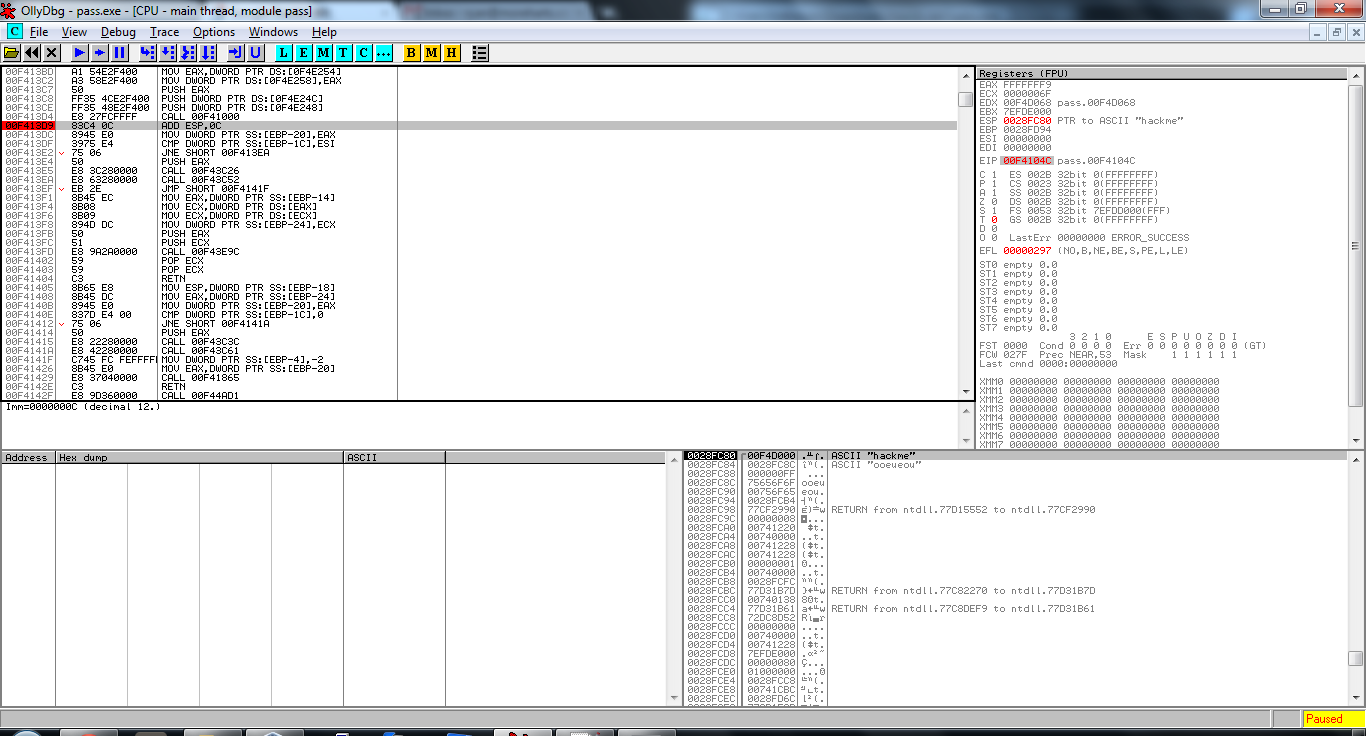
\includegraphics[width=1\textwidth]{breakpoint}
\caption{Breakpoint}
\label{fig:breakpoint}
\end{figure}

\begin{figure}[backmefound]
\centering
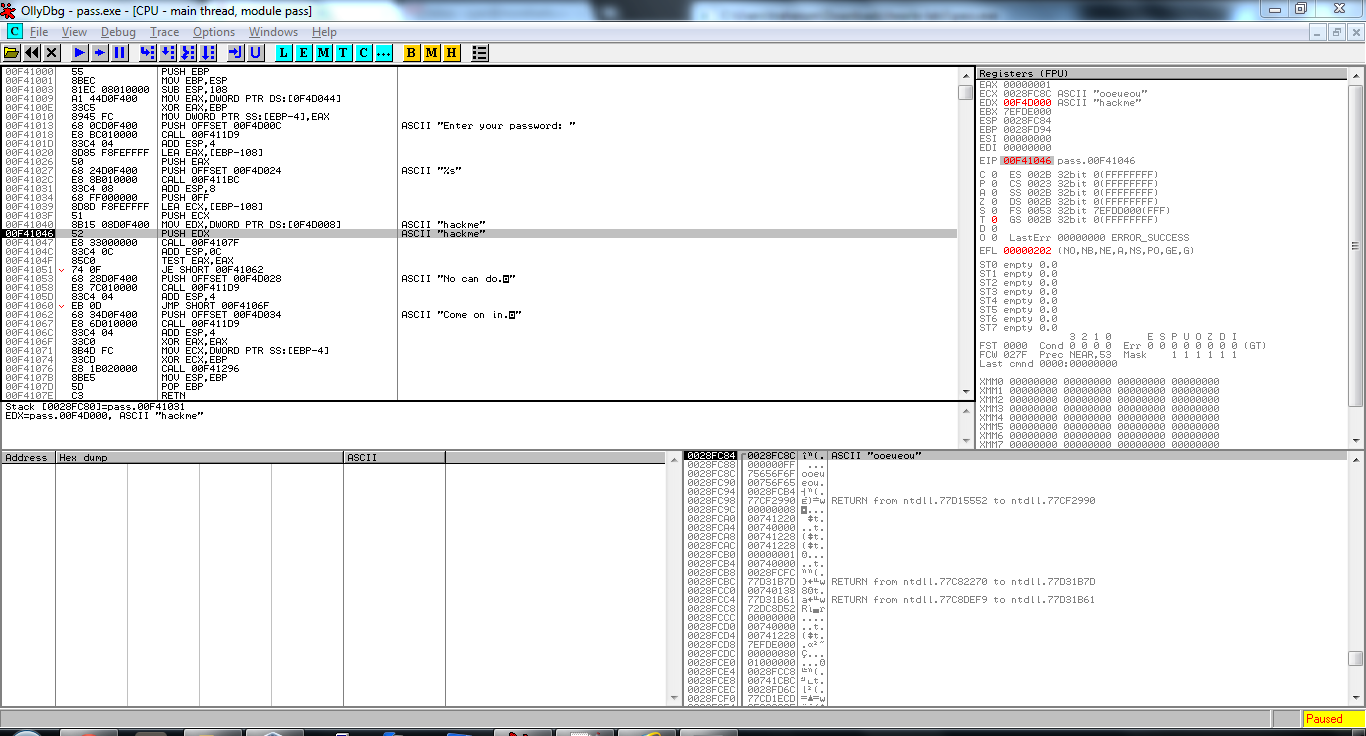
\includegraphics[width=1\textwidth]{hackmefound}
\caption{Password Found}
\label{fig:hackmefound}
\end{figure}

\subsection{The Lesson}
\par We can see easily from this task how difficult it is to secrets within the code itself. In this case, even a one-way hash on the stored password would have made the task much more difficult. The hash could have been extracted, but the attacker would need to brute force the actual password (or have a rainbow table entry for it).

\par On top of that, the hash really should be stored external to the program itself, such as in a database. An outside service can then provide a simple success or failure response to the program given a certain password. If the store is still on the local computer, however, the same problems exist. Ideally the password store is on another system, requiring the attacker to break into there to obtain the hash.

\FloatBarrier
\section{Task 2 - nmap}
\subsection{Scan}
\par For our scans of the two hosts we use the following switches:
\begin{description}\itemsep-2pt
	\item[-sV] Scan versions of services discovered
	\item[--version-all] Use all possible methods of version discovery, even unlikely ones
	\item[-O] Identify the OS and version
\end{description}

\par The output from nmap is show below:
\lstset{breaklines=true, title={nmap -sV --version-all -O}}
\lstinputlisting{nmap_output.txt}

\subsection{Analysis}
Host 1 (10.1.2.7) appears to be a Linux machine with a 2.6 kernel. It has several services running, including:
\begin{itemize}
	\item 22 - OpenSSH 5.8
	\item 80/443/5000/5001/7001 - Apache 2.2.17 (HTTP and HTTPS)
	\item 137/445 - SMB 3
	\item 515 - "printer," what's behind it is unknown
	\item 548 - Apple File Protocol, possibly
	\item 631 - CUPS 1.4 (printing)
	\item 873 - hp-pjl - "unknown fingerprint" for nmap though
	\item 5432 - PostgreSQL, unknown version
\end{itemize}

\par As a hacker, the version info might let us find a known vulnerability for each service. We also know that this host hosts files and/or printers, so breaking
into it may allow us to read sensitive information. Visiting the various http
ports in a browser would give us more info about the server's purpose and likely
give us a clue into what the database holds. Given the number of HTTP ports exposed, some of the higher ones may also be a development sites, which
may have more vulnerabilities than the production versions sitting at ports 80/443.
\\
\par Host 2 (10.1.2.24) appears to be a Windows 2003 box, although the exact service pack count not be determined. The following services exist:
\begin{itemize}
	\item 135 - MS RPC
	\item 139 - Netbios
	\item 445 - Samba
	\item 1025 - MS RPC
	\item 3389 - Terminal Service
\end{itemize}

\par We get less version information for individual services in this scan, but knowing that it's Windows 2003 narrows things down. Other than Terminal Service,
all of the exposed ports are well-known for having massive vulnerabilities. We
gain fairly limited knowledge of what this system is actually used for from the scan, but the exposed TS might indicate people remote into the box and may
leave sensitive work files.
\end{document}

